\documentclass[10pt,a4paper]{article}
\usepackage[latin1]{inputenc}
\usepackage{amsmath}
\usepackage{amsfonts}
\usepackage{amssymb}
\usepackage{graphicx}
\usepackage{hyperref}
% \usepackage{courier}
\usepackage{placeins}
\usepackage{fancyhdr}
\usepackage{color}
% \usepackage{xcolor}
\usepackage{listings}
\usepackage{geometry}
\usepackage{tabularx}
\usepackage[table]{colortbl}
\usepackage{placeins}
\usepackage{cite}
\usepackage{subcaption}
\usepackage{lipsum}
\usepackage{titlesec}
\usepackage[skip=8pt,labelfont=bf, font=sf]{caption}
	\DeclareCaptionFont{myfont}{\fontfamily{\sfdefault}\selectfont}

\hypersetup{
	colorlinks   = True,
	citecolor    = blue,
	linkcolor	 = blue,
}

% \geometry{letterpaper, portrait, margin=1in}
% \geometry{a4paper,margin=15mm,bindingoffset=25mm,heightrounded,}
\geometry{a4paper,margin=25mm}

\usepackage[dvipsnames]{xcolor}
\definecolor{lightgray}{rgb}{.93,.93,.93}
\definecolor{darkgray}{rgb}{.4,.4,.4}
\definecolor{purple}{rgb}{0.65, 0.12, 0.82}

\usepackage{helvet}
\usepackage{times}

\titleformat{\chapter}[display]
  {\normalfont\sffamily\huge\bfseries} % \color{blue}
  {\chaptertitlename\ \thechapter}{20pt}{\Huge}
\titleformat{\section}
  {\normalfont\sffamily\huge\bfseries} % \color{cyan}
  {\thesection}{1em}{}
 \titleformat{\subsection}
  {\normalfont\sffamily\Large\bfseries} % \color{cyan}
  {\thesubsection}{1em}{}
 \titleformat{\subsubsection}
  {\normalfont\sffamily\large\bfseries} % \color{cyan}
  {\thesubsubsection}{1em}{}
\renewenvironment{abstract}
 {\par\noindent\Huge\textbf{\abstractname.}\\\vspace{1em}\ignorespaces}
 {\par\medskip} 

% \renewcommand*\abstractname{Abstract\hfill}
% \renewcommand{\familydefault}{\sfdefault}


\def \lineheight {1.5pt}

\makeatletter
   \def\vhrulefill#1{\leavevmode\leaders\hrule\@height#1\hfill \kern\z@}
\makeatother

\usepackage{caption}
    \DeclareCaptionType{mycapequ}[][List of equations]
    \captionsetup[mycapequ]{labelformat=empty}

\usepackage{inconsolata}

\lstset{
	language=Matlab,
	backgroundcolor=\color{lightgray},
	keywordstyle=\color{blue}\bfseries,
	stringstyle=\color{red}\ttfamily,
	commentstyle=\color{ForestGreen}\ttfamily,
	identifierstyle=\color{black},
	extendedchars=true,
	% basicstyle=\footnotesize\ttfamily,
	basicstyle=\normalsize\fontencoding{T1}\ttfamily,
	showstringspaces=false,
	showspaces=false,
	numbers=left,
	numberstyle=\footnotesize,
	numbersep=9pt,
	tabsize=2,
	breaklines=true,
	showtabs=false,
	captionpos=b
}

\lstset{
	language=Python,
	backgroundcolor=\color{lightgray},
	keywordstyle=\color{blue}\bfseries,
	stringstyle=\color{red}\ttfamily,
	commentstyle=\color{ForestGreen}\ttfamily,
	identifierstyle=\color{black},
	extendedchars=true,
	% basicstyle=\footnotesize\ttfamily,
	basicstyle=\normalsize\fontencoding{T1}\ttfamily,
	showstringspaces=false,
	showspaces=false,
	numbers=left,
	numberstyle=\footnotesize,
	numbersep=9pt,
	tabsize=2,
	breaklines=true,
	showtabs=false,
	captionpos=b
}

\fancypagestyle{firstpage}{%
  \fancyhf{}% clear default for head and foot
  % \rfoot{\textbf{Page \thepage}}
  % \lfoot{\textbf{\today}}
  \renewcommand{\headrulewidth}{0pt}
}
\fancypagestyle{blank}{%
	\fancyhf{}
	\renewcommand{\headrulewidth}{0pt}
}

\fancypagestyle{nohdr}{%
	\fancyhf{}
	\renewcommand{\headrulewidth}{0pt}
	\rfoot{\fontfamily{\sfdefault}\selectfont\textbf{Page \thepage}}
}

\renewcommand{\headrulewidth}{1pt}% 2pt header rule
\pagestyle{fancy}
\fancyhf{}
\rhead{\fontfamily{\sfdefault}\selectfont \textbf{Specialization Project}}
\lhead{\fontfamily{\sfdefault}\selectfont \textbf{\leftmark}}
\rfoot{\fontfamily{\sfdefault}\selectfont \textbf{Page \thepage}}
\lfoot{\fontfamily{\sfdefault}\selectfont \textbf{Cole Nielsen}} % \today




\title{\textbf{Simulation, Design and Measurement of Branchline \\ Microstrip Directional Coupler\\}}
\date{}

% \date{}
\sloppy\raggedright
\begin{document}	
	% \maketitle 
	% \renewcommand{\familydefault}{\sfdefault}
	\thispagestyle{firstpage}
	\fontfamily{\sfdefault}\selectfont 
	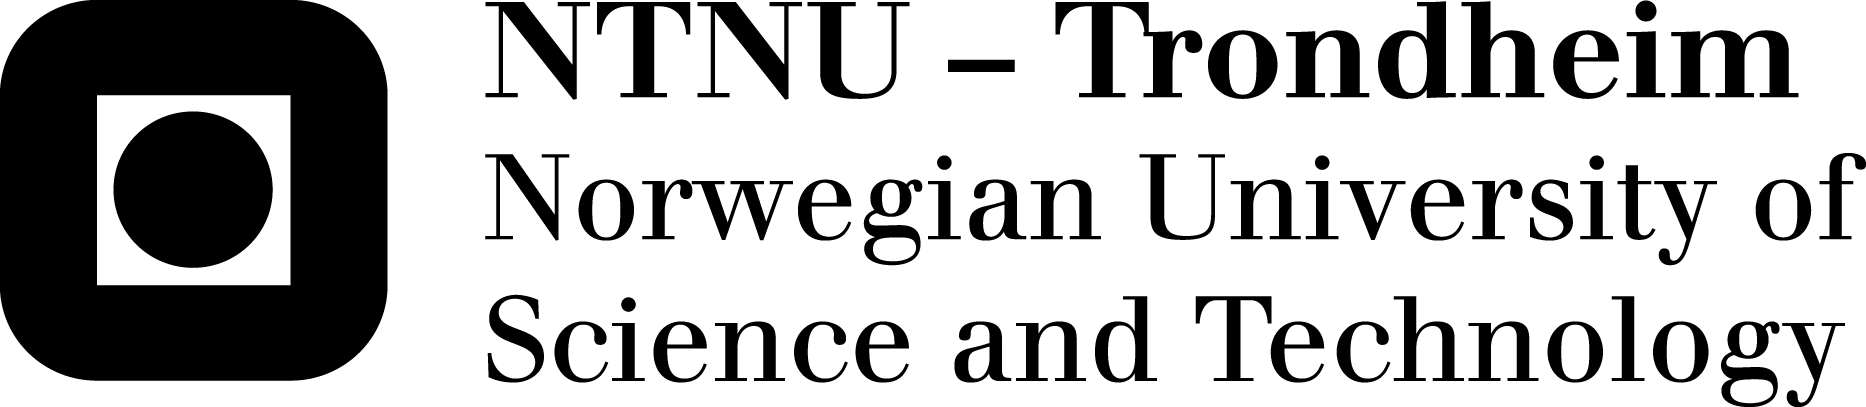
\includegraphics[width=0.5\linewidth]{logo_ntnu_eng_black.png} \\
	\vspace{8em}
	\huge Ultra-low power PLL frequency sythesizer for Wake-Up Receiver applications\\	
	\vspace{3em}
	\huge \textbf{Cole Nielsen}\\
	\vspace{14em}
	\large
	Electronic Systems Design, Specialization Project\\
	\vspace{4pt}
	\FloatBarrier

	\def\arraystretch{1.3}
	\setlength{\tabcolsep}{1em}
	\begin{tabular}{@{} l  l}
	Submission date: & December 2019\\
	Supervisor: & Trond Ytterdal, IET\\
	Co-supervisor: & Carsten Wulff, IET\\
	\end{tabular} \\
	\FloatBarrier
	\vspace{3em}
	Norwegian University of Science and Technology \\ 
	\vspace{4pt}Department of Electronic Systems\\
	
	% \begin{center}
	% 	\large
	% 	\begin{tabular}{ l r }
	% 		\textbf{Name} & Cole Nielsen \\
	% 		\textbf{Assigned N$^\textbf{\textnormal{o}}$} & 13 \\
	% 		\textbf{Term} & Autumn 2018\\
	% 		\textbf{Instructor} & Guennadi Kouzaev\\
	% 	\end{tabular}
	% \end{center}
	% \vspace{2em}
	% \vhrulefill{\lineheight}
	\pagebreak
	\thispagestyle{blank}
	\null\pagebreak

	% % % % % % % % % % % % % % % % % % % % % % % % % % % % % % % % % % % % 
	% Abstract		
	\setcounter{page}{1}
	\pagebreak
	\thispagestyle{nohdr}
	\begin{abstract}
		\large\fontfamily{\rmdefault}\selectfont 
		\noindent\lipsum[1]
	\end{abstract}
	% \section*{Abstract}
	% fjdsfkajjlkf

	% % % % % % % % % % % % % % % % % % % % % % % % % % % % % % % % % % % % 
	% Project Description
	\pagebreak
	\thispagestyle{nohdr}
	\null\pagebreak
	\thispagestyle{nohdr}
	\Huge\textbf{Problem description.}\\
	\vspace{1em}
	\large\fontfamily{\rmdefault}\selectfont 
	\lipsum[1]

	% % % % % % % % % % % % % % % % % % % % % % % % % % % % % % % % % % % % 
	% Preface
	\pagebreak
	\thispagestyle{nohdr}
	\null\pagebreak
	\thispagestyle{nohdr}
	\large\fontfamily{\sfdefault}\selectfont 
	\Huge\textbf{Preface.}\\
	\vspace{1em}
	\large\fontfamily{\rmdefault}\selectfont 
	\lipsum[1]

	% % % % % % % % % % % % % % % % % % % % % % % % % % % % % % % % % % % % 
	% Contents	
	\fontfamily{\sfdefault}\selectfont 
	\pagebreak
	\tableofcontents
	\pagebreak
	\listoffigures
	\listoftables

	% \vhrulefill{\lineheight}

	\fontfamily{\rmdefault}\selectfont 
	% % % % % % % % % % % % % % % % % % % % % % % % % % % % % % % % % % % % 
	% Abbreviations
	\pagebreak
	% \thispagestyle{nohdr}
	\null\pagebreak
	\section*{Abbreviations.}

	\begin{tabular}{@{}ll}
		\textbf{\textsf{DAC}}& 	Digital-to-analog converter\\
		\textbf{\textsf{DCO}}& 	Digitally controlled oscillator\\
		\textbf{\textsf{FDSOI}} &  Fully-depleted silicon on insulator	\\
		\textbf{\textsf{FET}} &  Field effect transistor	\\
		\textbf{\textsf{FSK}} &  Frequency-shift keying	\\
		\textbf{\textsf{PLL}} &  Phase locked loop	\\
		\textbf{\textsf{RO}}& 	Ring-oscillator\\
		\textbf{\textsf{RX}}& 	Receiver\\
		\textbf{\textsf{SSB}}& 	Single side band\\
		\textbf{\textsf{TDC}}& 	Time-to-digital converter \\
		\textbf{\textsf{TSPC}}& 	True single-phase circuit\\
		\textbf{\textsf{VCO}}& 	Voltage controlled oscillator\\
		\textbf{\textsf{WURX}}& 	Wake-up receiver\\
		& 	\\
		& 	\\
	\end{tabular}


	% % % % % % % % % % % % % % % % % % % % % % % % % % % % % % % % % % % % 
	% WAVEGUIDE MEASUREMENTS LAB
	\pagebreak
	\FloatBarrier
    \section{Introduction}

    \section{Methods}

    \section{Results}

    \section{Discussion}

	% % % % % % % % % % % % % % % % % % % % % % % % % % % % % % % % % % % % 
    \FloatBarrier
    \section{Conclusion}
    \lipsum[1]


	% % % % % % % % % % % % % % % % % % % % % % % % % % % % % % % % % % % % 
	\section{Block diagram}
		\center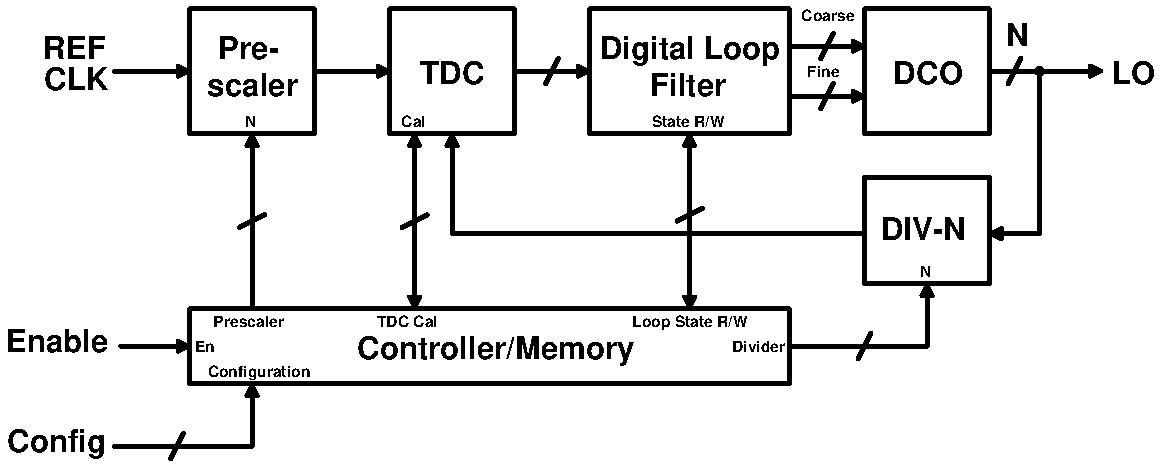
\includegraphics[width=0.75\textwidth, angle=0]{figs/pll2.pdf}
		\vspace{-.1em}
		\begin{table}[htb!]
			\tiny
			\centering
			\def\arraystretch{1.5}		
			\setlength\arrayrulewidth{0.75pt}
			\setlength{\tabcolsep}{1em} % for the horizontal padding
			\begin{tabular}{|l|l|l|l|l|}
				\hline 
				\rule[-1ex]{0pt}{2.5ex} \cellcolor{gray!40}\textbf{DCO} & \cellcolor{gray!40}\textbf{TDC} & \cellcolor{gray!40}\textbf{Divider }& \cellcolor{gray!40}\textbf{Other} & \cellcolor{gray!40}\textbf{SUM} \\ 
				\hline 
				\rule[-1ex]{0pt}{2.5ex} 70 $\mu$W& 20 $\mu$W & 10 $\mu$W & $<<$ 1 $\mu$W & 100 $\mu$W\\ 
				\hline 
			\end{tabular} 
			% \caption{Assigned specifications for branch line hybrid design.}
			% \label{asgn_specs}
		\end{table}   

	\section{Specifications}
		\scriptsize
		\begin{table}[h!]
			\centering
			\def\arraystretch{1.5}		
			\setlength\arrayrulewidth{0.75pt}
			\setlength{\tabcolsep}{1em} % for the horizontal padding
			\begin{tabular}{|l|r|l|l|}
				\hline 
				\rule[-1ex]{0pt}{2.5ex} \cellcolor{gray!40}\textbf{Parameter} & \cellcolor{gray!40}\textbf{Value} & \cellcolor{gray!40}\textbf{Unit }& \cellcolor{gray!40}\textbf{Notes}\\ 
				\hline 
				\rule[-1ex]{0pt}{2.5ex} \textbf{Frequency}  & 2.4-2.4835 & GHz & 2.4G ISM Band\\ 
				\hline 
				\rule[-1ex]{0pt}{2.5ex} \textbf{Ref. frequency} & 16 & MHz & Yields 6 channels \\ 
				\hline 
				\rule[-1ex]{0pt}{2.5ex} \textbf{Power} & $\leq$ 100  &$\mu$W & \\ 
				\hline 
				\rule[-1ex]{0pt}{2.5ex} \textbf{Residual FM} & $\leq$ 107  &kHz$_{RMS}$ & BER $\leq$ 1e-2, $f_{dev}$=$\pm$250 KHz\\ 
				\hline 
				\rule[-1ex]{0pt}{2.5ex} \textbf{Initial Lock Time} & $\leq$ 50 & $\mu$s & Upon cold start \\ 
				\hline 
				\rule[-1ex]{0pt}{2.5ex} \textbf{Re-lock Time} & $\leq$ 5 & $\mu$s & Coming out of standby \\ 
				\hline 
				\rule[-1ex]{0pt}{2.5ex} \textbf{Bandwidth} & 100 & kHz & (nominally), tunable \\ 
				\hline 
			\end{tabular} 
			% \caption{Assigned specifications for branch line hybrid design.}
			% \label{asgn_specs}
			\caption{System-level specifications}
		\end{table}   
		Additionally: PLL output should support IQ sampling at LO frequency.

		\scriptsize
		\begin{table}[h!]
			\centering
			\def\arraystretch{1.5}		
			\setlength\arrayrulewidth{0.75pt}
			\setlength{\tabcolsep}{1em} % for the horizontal padding
			\begin{tabular}{|l|r|l|l|}
				\hline 
				\rule[-1ex]{0pt}{2.5ex} \cellcolor{gray!40}\textbf{Parameter} & \cellcolor{gray!40}\textbf{Value} & \cellcolor{gray!40}\textbf{Unit }& \cellcolor{gray!40}\textbf{Notes}\\ 
				\hline 
				\rule[-1ex]{0pt}{2.5ex} \textbf{DCO LSB Resolution}  & $\leq$ 50  & kHz & Determined from quantization noise.\\ 
				\hline 
				\rule[-1ex]{0pt}{2.5ex} \textbf{DCO DNL} & < 1 & LSB & Ensures monotonicity \\ 
				\hline 
				\rule[-1ex]{0pt}{2.5ex} \textbf{TDC Resolution} & $\leq$ 3.8  & ns & \\ 
				\hline 
				\rule[-1ex]{0pt}{2.5ex} \textbf{TDC Resolution (bits)} & $\geq$ 4.03 &bits & \\ 
				\hline 
			\end{tabular} 
			\caption{Component-level specifications.}
			% \caption{Assigned specifications for branch line hybrid design.}
			% \label{asgn_specs}
		\end{table}   

	\FloatBarrier
	\flushleft
	\section{DCO tuning}
	\subsection{Backgate tuning}
	\normalsize
	Tuning of a ring oscillator DCO through backgate terminal control will be considered. A general analysis of ring oscillator frequency will be made first to begin.

	\subsection{Ring oscillator frequency derivation}
	To analyze the oscillation frequency of a CMOS ring oscillator, an approximate model for a CMOS inverter will first be considered. A common model for delay in digital circuits [elmore delay model] is an RC circuit, where the MOSFET channels are approximated with an average conductance value $\langle g_{ch} \rangle$, and the output node is approximated to have a capacitance of C. With such a model, a ring oscillator would be assumed to have waveforms as decaying exponential, with time constant $\tau = \langle g_{ch} \rangle^{-1}C$, such as in Figure \ref{fig:rosc_rc}.
	\begin{figure}[htb!]
		\center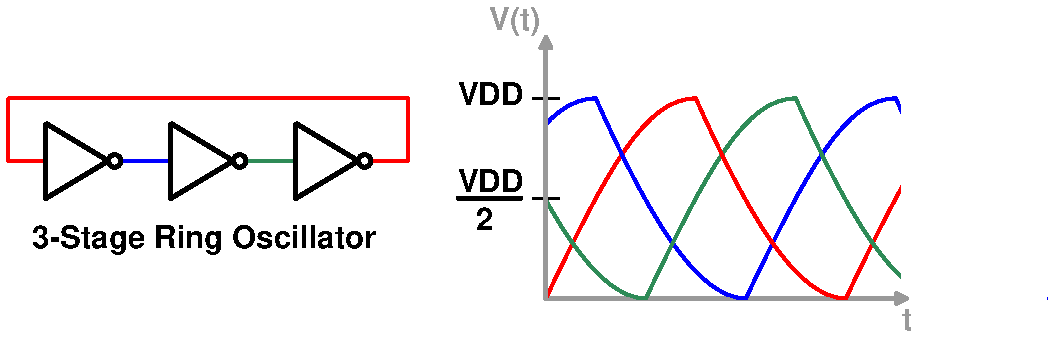
\includegraphics[width=0.8\linewidth, angle=0]{figs/inv_waves3.pdf}
		\caption{Model for ring oscillator.}
		\label{fig:rosc_rc}
	\end{figure}

	\begin{figure}[htb!]
        \centering
        \begin{subfigure}{.5\textwidth}
            \centering
            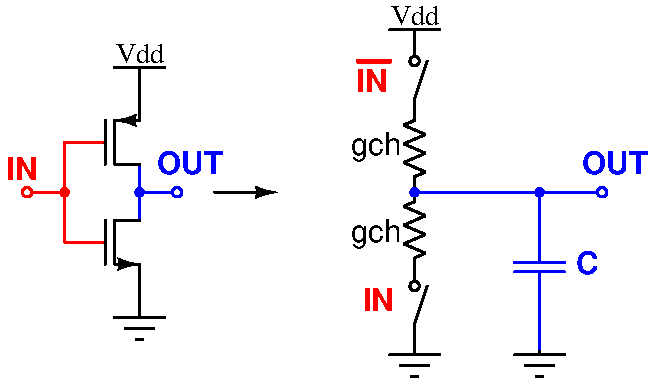
\includegraphics[width=\linewidth]{figs/inv_rc_model.pdf}
            \caption{Inverter approximate model.}
            \label{fig:rosc_3stg_cir}
        \end{subfigure}%
        \begin{subfigure}{.5\textwidth}
            \centering
            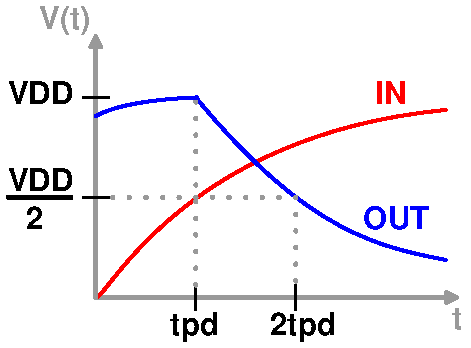
\includegraphics[width=0.8\linewidth]{figs/inv_waves2.pdf}
            \caption{Inverter waveforms in ring oscillator.}
            \label{fig:rosc_3stg_wave}
        \end{subfigure}
        \caption{Approximate model for ring oscillator inverter delay cell.}
        \label{fig:rosc_3stg}
    \end{figure}

	To calculate oscillation frequency ring oscillator from the RC model, several inferences are made:
	\begin{itemize}
		\item The switching point $V_M$ of the inverters is $V_{DD}/2$, based on the assumption that the NMOS and PMOS are of equal strength.
		\item The output of an inverter will have a decaying exponential which starts coincident with the passing of $V_M$ at the input.
		\item The propagation delay $t_{pd}$ for an inverter will be the time differential between the $V_M$ crossing points on the input and output.
		\item The oscillator frequency will be $f_{osc}$ = $1/2Nt_{pd}$, where N is the number of stages.
	\end{itemize}
	Following the definition of $V_M$, it is trivial to find that $t_{pd}$ = $\tau\ln2$. It is therefore known that:
	\begin{equation}
	f_{osc} = \frac{1}{2Nt_{pd}} = \frac{\langle g_{ch}\rangle}{2\ln(2)NC}
	\end{equation}
	The node capacitance C is trivial to find based on the inverter gate capacitance:
	\begin{equation}
		C = C_{ox}\left ( W_N L_N + W_P L_N \right)
	\end{equation}
	The average channel conductance $\langle g_{ch} \rangle$ is more involved to find. To do so, several assumptions are made:
	\begin{itemize}
		\item L $>>$ L$_{min}$, so no velocity saturation, and therefore square law is applicable.
		\item NMOS and PMOS have equal $V_t$ and transconducance.
		\item Output transition occur with the active FET in saturation during $t_{pd}$. This requires:
		\begin{itemize}
			\item $V_{DD}/4 < V_{t} < V_{DD}/2$
		\end{itemize}
	\end{itemize}
	Following those assumptions, $\langle g_{ch} \rangle$ can be computed via integral within the period $t_{pd}$:
	\begin{equation}
		\langle g_{ch} \rangle = \frac{1}{t_{pd}} \int_0^{t_{pd}}\frac{I_{out}(t)}{V_{out}(t)}dt
	\end{equation}
	$I_{out}$ is computed using the saturated MOSFET square law model an exponential waveforms assumptions. An $I_{short}$ term is included to account for output current reduction from short-circuit conduction.
	\begin{equation}
	I_{out}(t) = \frac{k_n}{2}\left(\frac{W}{L}\right)_n\left[\left(V_{in}(t) - V_t\right)^2 \right]  - I_{short} = \frac{k_n}{2}\left(\frac{W}{L}\right)_n\left[\left(V_{DD}\left(1-e^{-t/\tau}\right) - V_t\right)^2 - \left(\frac{V_{DD}}{2} -V_t\right)^2\right]
	\end{equation}
	$k_n = \mu_nC_{ox}$, with the equal PMOS/NMOS assumption, $k_n\left(\frac{W}{L}\right)_n=k_p\left(\frac{W}{L}\right)_p$. $V_{out}$ is simply a decaying exponential with a delay $t_pd$ versus the input:
	\begin{equation}
	V_{out} = V_{DD}e^{-(t-t_{pd})/\tau}
	\end{equation}
	Now, computing the integral for $\langle g_{ch} \rangle$ yields:
	\begin{equation}
		\langle g_{ch} \rangle = \frac{1}{2}\mu_nC_{ox}\left(\frac{W}{L}\right)_n\left[V_{DD}\left(\frac{7}{8\ln2}-1\right)-V_t\left(\frac{1}{\ln2}-1\right) \right]
	\end{equation}
	Solving for oscillator frequency:
	\begin{equation}
		f_{osc} = \frac{\mu_nC_{ox}}{4\ln2NC}\left(\frac{W}{L}\right)_n\left[V_{DD}\left(\frac{7}{8\ln2}-1\right)-V_t\left(\frac{1}{\ln2}-1\right) \right]
	\end{equation}
	If gate capacitance is the dominant load component:
	\begin{equation}
		f_{osc} = \frac{\mu_n}{8\ln2N}\cdot\frac{1}{L^2}\left[V_{DD}\left(\frac{7}{8\ln2}-1\right)-V_t\left(\frac{1}{\ln2}-1\right) \right]
	\end{equation}
	Power can also be calculated, knowing in digital circuits $P = fCV_{DD}^2$, thus:
	\begin{equation}
		P_{osc} = Nf_{osc}CV_{DD}^2 = \frac{\mu_nC_{ox}}{4\ln2}\left(\frac{W}{L}\right)_n\left[V_{DD}\left(\frac{7}{8\ln2}-1\right)-V_t\left(\frac{1}{\ln2}-1\right) \right]
	\end{equation}
	It should be noted that the most significant factor for power consumption is FET aspect ratio (W/L).

	\subsection{Ring oscillator backgate tuning derivation}
	Using the basic expressions for ring oscillator frequency, the operature under backgate biasing can be found. In UTBB-FDSOI processes, the threshold voltage of a FET varies with linear dependence on the applied back gate bias $V_{BG}$ (relative to source). Given the body effect coefficient of a process, $\gamma$, $V_t$ is:
	\begin{equation}
		V_t = V_{t0} - \gamma V_{BG}
	\end{equation}
	Using this in the ring oscillator frequency equation:
	\begin{equation}
		f_{osc} = \frac{\mu_nC_{ox}}{4\ln2NC}\left(\frac{W}{L}\right)_n\left[V_{DD}\left(\frac{7}{8\ln2}-1\right)-V_{t0}\left(\frac{1}{\ln2}-1\right) + \gamma V_{BG}\left(\frac{1}{\ln2}-1\right) \right]
	\end{equation}
	Equivalently, $f_{osc} = f_{0,osc} + \Delta f_{osc}(V_{BG})$, where:
	\begin{equation}
		\Delta f_{osc}(V_{BG}) = \gamma V_{BG}\frac{\mu_nC_{ox}}{4\ln2NC}\left(\frac{W}{L}\right)_n\left[\frac{1}{\ln2}-1\right]
	\end{equation}	
	And $f_{0,osc}$ is the frequency with no backgate bias. If the backgate is swept from 0 to $V_{DD}$, and the node capacitance is increasingly varied (C0 to C3), Figure \ref{fig:rosc_tuning} is observed. Note that the change in frequency is linear with to backgate bias.
	\FloatBarrier
	\begin{figure}[htb!]
		\center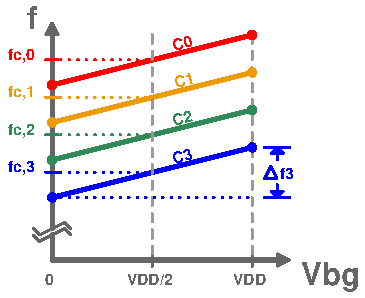
\includegraphics[width=0.3\linewidth, angle=0]{figs/backgate_rosc_tuning2.pdf}
		\caption{Backgate-tuned ring oscillator with coarse tuning capacitor bank.}
		\label{fig:rosc_tuning}
	\end{figure}
	If the backgate voltage is constrained in the range [0, $V_{DD}$], the center frequency $f_c$ in the tuning range of the oscillator is then:
	\begin{equation}
		f_{c} = \frac{\mu_nC_{ox}}{4\ln2NC}\left(\frac{W}{L}\right)_n\left[V_{DD}\left(\frac{7}{8\ln2}-1+\frac{\gamma}{2\ln2}-\frac{\gamma}{2}\right)-V_{t0}\left(\frac{1}{\ln2}-1\right)\right]
	\end{equation}
	The tuning range is also therefore:
	\begin{equation}
		\Delta f = \frac{\gamma V_{DD}}{2}\frac{\mu_nC_{ox}}{4\ln2NC}\left(\frac{W}{L}\right)_n\left[\frac{1}{\ln2}-1\right]
	\end{equation}
	The fractional tuning range of the oscillator is:
	\begin{equation}
		\frac{\Delta f}{f_c} = \frac{1}{2}\cdot\frac{\gamma V_{DD}\left( 1-\ln2 \right)}{V_{DD}\left(\frac{7}{8}-\ln2+\frac{\gamma}{2}-\frac{\gamma}{2}\ln2\right)-V_{t0}\left(1-\ln2\right)}
	\end{equation}	
	If a N-bit DAC is used to control the oscillator, the resulting DCO gain is therefore:
	\begin{equation}
		K_{DCO} = \frac{\Delta f}{2^{N_{DAC}}} = \frac{f_c}{2^{N_{DAC}+1}}\cdot\frac{\gamma V_{DD}\left( 1-\ln2 \right)}{V_{DD}\left(\frac{7}{8}-\ln2+\frac{\gamma}{2}-\frac{\gamma}{2}\ln2\right)-V_{t0}\left(1-\ln2\right)}
	\end{equation}	
	\subsection{DCO Gain Uncertainty}
	The DCO gain $K_{DCO}$ is used in setting the loop filter coefficients, so the uncertainty of the DCO gain is of interest to allow for statistical analysis of the PLL across process variation. The uncertainty of $K_{DCO}$ (normalized with nominal $K_{DCO}$ value) as a function of $V_{DD}$, $V_{t0}$ and $\gamma$ is:
	\begin{equation}
		\sigma_{KDCO} = \sqrt{\left(\frac{\partial K_{DCO}}{\partial V_{DD}}\cdot\frac{\sigma_{VDD}}{K_{DCO}} \right)^2 + \left(\frac{\partial K_{DCO}}{\partial V_{t0}}\cdot\frac{\sigma_{Vt0}}{K_{DCO}} \right)^2 + \left(\frac{\partial K_{DCO}}{\partial \gamma}\cdot\frac{\sigma_\gamma}{K_{DCO}} \right)^2}
	\end{equation}

	\begin{equation}
		\frac{\partial K_{DCO}}{\partial V_{DD}} = \frac{f_c}{2^{N_{DAC}+1}}\cdot\frac{-\gamma V_{t0}(1-\ln2)^2}{\left[ V_{DD}\left(\frac{7}{8}-\ln2+\frac{\gamma}{2}-\frac{\gamma}{2}\ln2\right)-V_{t0}\left(1-\ln2\right) \right]^2}
	\end{equation}
	\begin{equation}
		\frac{\partial K_{DCO}}{\partial V_{t0}} = \frac{f_c}{2^{N_{DAC}+1}}\cdot\frac{\gamma V_{DD}(1-\ln2)^2}{\left[ V_{DD}\left(\frac{7}{8}-\ln2+\frac{\gamma}{2}-\frac{\gamma}{2}\ln2\right)-V_{t0}\left(1-\ln2\right) \right]^2}
	\end{equation}
	\begin{equation}
		\frac{\partial K_{DCO}}{\partial \gamma} = \frac{f_c}{2^{N_{DAC}+1}}\cdot\frac{V_{DD}\cdot(1-\ln2) \left[ V_{DD}\left(\frac{7}{8}-\ln2\right)-V_{t0}\left(1-\ln2\right) \right]}{\left[ V_{DD}\left(\frac{7}{8}-\ln2+\frac{\gamma}{2}-\frac{\gamma}{2}\ln2\right)-V_{t0}\left(1-\ln2\right) \right]^2}
	\end{equation}
	Simplified:
	\begin{multline}
		\sigma_{KDCO} = \frac{1}{\gamma V_{DD} \left[ V_{DD}\left(\frac{7}{8}-\ln2+\frac{\gamma}{2}-\frac{\gamma}{2}\ln2\right)-V_{t0}\left(1-\ln2\right) \right]}\cdot\\ \sqrt{\left(\gamma V_{t0} (1-\ln2)\sigma_{VDD} \right)^2 + \left(\gamma V_{DD} (1-\ln2)\sigma_{Vt0} \right)^2 + \left( V_{DD}\left[ V_{DD}\left(\frac{7}{8}-\ln2\right)-V_{t0}\left(1-\ln2\right) \right]\sigma_{\gamma} \right)^2 }
	\end{multline}		

	\FloatBarrier
	\section{pres1}
		\subsection{Motivation}
		\begin{itemize}
			\footnotesize
			\item WSNs require ultra-low power circuits. A sensor should last for many years (>5) on a coin cell battery.
			\item With the below $P_{avg}$ values, a CR2032 cell with 0.6 Wh capacity will last:
			\begin{itemize}
				\scriptsize
				\item 1 $\mu$W $\rightarrow$ 70 years
				\item 10 $\mu$W $\rightarrow$ 7 years
				\item 100 $\mu$W $\rightarrow$ 0.7 years
			\end{itemize} 
			\item To save power, run devices with low duty cycle; activate remotely using wake up receiver (WuRx).
			\begin{itemize}
				\scriptsize
				\item For 5 years of life, using 10\% of battery energy for the WuRx, \textbf{$P_{WURX}$ < 1.4 $\mu$W} on average is required.
			\end{itemize} 
			\item Main challenge for receiver is low power LO synthesis.
			\begin{itemize}
				\scriptsize
				\item Synthesizer-free approaches (OOK receiver) lack robustness.
				\item Advanced modulation schemes are too demanding with phase noise (PN).
				\item Best option is FSK, using low power synthesizer with loose PN requirements to meet power target.
			\end{itemize} 
		\end{itemize}  

		\flushleft
		\subsection{State of the Art}
		\footnotesize
		Performance averages based on sampling of 15 works published in IEEE:
		\scriptsize
		\vspace{-1em}
		\begin{table}[htb!]
			\tiny
			\centering
			\def\arraystretch{1.5}		
			\setlength\arrayrulewidth{0.75pt}
			\setlength{\tabcolsep}{1em} % for the horizontal padding
			\begin{tabular}{|l|l|l|l|l|l|l|l|}
				\hline 
				\rule[-1ex]{0pt}{2.5ex} \cellcolor{gray!40}\textbf{Group} & \cellcolor{gray!40}\textbf{Count} & \cellcolor{gray!40}\textbf{Power [$\mu$W] }& \cellcolor{gray!40}\textbf{Freq [MHz]} & \cellcolor{gray!40}\textbf{RF BW [MHz]}& \cellcolor{gray!40}\textbf{Bitrate [kbps]}& \cellcolor{gray!40}\textbf{BER }& \cellcolor{gray!40}\textbf{Sens. [dBm]}\\ 
				\hline 
				\rule[-1ex]{0pt}{2.5ex} \textbf{All} & 15 & 96 & 1400 & 1.2 & 52 & 3e-3 & -66\\ 
				\hline 
				\rule[-1ex]{0pt}{2.5ex} \textbf{800/900M} & 6 & 138 & 887 & 0.95 & 15 & 4e-3 & -68\\ 
				\hline 
				\rule[-1ex]{0pt}{2.5ex} \textbf{All 2.4G} & 6 & 81 & 2400 & 2 & 60 & 2.8e-3 & -67\\ 
				\hline 
				\rule[-1ex]{0pt}{2.5ex} \textbf{2.4G FSK} & 2 & 190 & 2400 & 1.5 & 98 & 1e-3 & -69\\ 
				\hline 
				\rule[-1ex]{0pt}{2.5ex} \textbf{2.4G OOK} & 4 & 27 & 2400 & 2.5 & 41.5 & 4e-3 & -66\\ 
				\hline 
			\end{tabular} 
			% \caption{Assigned specifications for branch line hybrid design.}
			% \label{asgn_specs}
		\end{table}   
		\begin{itemize}
			\footnotesize
			\item State of art of 2.4G WuRx:
			\begin{itemize}
				\item Active Power $\leq$ 100 $\mu$W
				\item RF BW $\approx$ 1 MHz
				\item Sensitivity = -70 dBm (BER 1e-3)
				\item Data Rate = 100 kbps
			\end{itemize}
		\end{itemize}

		\flushleft
		\subsection{Objectives - Synthesizer goals}
		\begin{itemize}
			\footnotesize
			\item Design ultra-low-power frequency synthesizer to meet requirements for \textit{practical} wake up receivers.
			\begin{itemize}
				\footnotesize
				\item \textbf{$\leq$1 $\mu$W average consumption}
				\item Targeting \textbf{1\% duty cycle} for \textbf{$\leq$100 $\mu$W active power}.
				\begin{itemize}
					\item Fast locking to reduce on time/energy consumption.
				\end{itemize}
			\end{itemize} 
			\item Synthesis range within \textbf{2.4 GHz ISM band}.
			\item Enable \textbf{wake up call detection within 1s} with 1e-3 miss rate.
			\begin{itemize}
				\scriptsize
				\item Achievable with 250 kbps data, BER $\leq$ 1e-2, 1\% duty, 20\% wake up call Tx density.
				\item Assuming 32-symbol wake up call used for false-alarm robustness.
				\item High BER inherent due to high PN, expect many misses before sucess.  
				\item Use large FSK modulation index (m) to ease PN and power requirements. 
				\begin{itemize}
					\scriptsize
					\item m=2 $\rightarrow$ 2$\pi$ phase shift per symbol or $\pm$250 kHz frequency deviation.
					\item RMS Residual frequency modulation (RFM) of PLL should be $<<$ symbol frequency deviation to achieve desired BER.
					\item \textbf{RFM is derived from phase noise integration; use to constrain PLL PN.}
				\end{itemize}
			\end{itemize}      
		\end{itemize}

		\flushleft
		\subsection{Architecture - concepts}
		\begin{itemize}
			\footnotesize
			\item Utilize \textbf{Digital PLL}.\@ 
			\begin{itemize}
				\footnotesize
				\item Inherent feedback helps with PVT variation (yield).
				\item Calibration easy in digital design, agains helps with PVT variation.
				\item Can store state when PLL idle, allowing for faster lock times coming out of standby.
			\end{itemize}       
		  \item Utilize low duty cycle to achieve power target.     
			\begin{itemize}
				\footnotesize
				\item Can exploit semi-frequent calibration to improve performance.
				\item Possibly can run PLL open loop when lock is achieved to save power.
			\end{itemize} 
		  \item Utilize oscillator running at 1/N subharmonic of target frequency.
			\begin{itemize}
				\footnotesize
				\item Use 2N phases in oscillator to achieve equivalent IQ sampling.
				\item Avoids having to run oscillator at 2x target frequency as done typically.
				\item 1/3 subharmonic operation should allow for dual mode 2.4G and 915M operation.
			\end{itemize} 
			\item Employ subsampling to reduce divider noise and TDC power?
		\end{itemize}

		\flushleft
		\subsection{State of Art - Sub-1 mW PLLS}
		\footnotesize Application is niche, so comparable PLLs hard to find.
		\vspace{-1em}
		\begin{table}[htb!]
			\tiny
			\centering
			\def\arraystretch{1.5}		
			\setlength\arrayrulewidth{0.75pt}
			\setlength{\tabcolsep}{1em} % for the horizontal padding
			\begin{tabular}{|l|l|l|l|l|l|l|l|}
				\hline 
				\rule[-1ex]{0pt}{2.5ex} \cellcolor{gray!40}\textbf{Type} & \cellcolor{gray!40}\textbf{P$_{PLL}$ [$\mu$W]}& \cellcolor{gray!40}\textbf{P$_{osc}$ [$\mu$W] }& \cellcolor{gray!40}\textbf{Freq [MHz]} & \cellcolor{gray!40}\textbf{PN@$\Delta f$ [dBc/Hz]}& \cellcolor{gray!40}\textbf{t$_{lock}$* [$\mu$s]}& \cellcolor{gray!40}\textbf{Osc. }& \cellcolor{gray!40}\textbf{Ref Freq}\\ 
				\hline 
				\rule[-1ex]{0pt}{2.5ex} \textbf{Dig. Frac-N} & 650 & 304 & 2400 & -110@0.5M & 15/4 & LC & 26M\\ 
				\hline 
				\rule[-1ex]{0pt}{2.5ex} \textbf{Ana. Int-N }& 680 & 510 & 2400 & -110@1M & 130/70 & LC & 1M\\ 
				\hline 
				\rule[-1ex]{0pt}{2.5ex} \textbf{Ana. Int-N} & 128 &  & 500 & -94@1M &  & Ring & 31.25M\\ 
				\hline 
				\rule[-1ex]{0pt}{2.5ex} \textbf{Ana. Int-N} & 570 &  & 800 & -92.6@0.1M & 200 & LC & 0.2M\\ 
				\hline 
				\rule[-1ex]{0pt}{2.5ex} \textbf{Dig. Frac-N} & 250 & 173 & 2448 &  & 22/1 & Ring & 9M\\ 
				\hline 
				\rule[-1ex]{0pt}{2.5ex} \textbf{Ana. Int-N} & 950 &  & 5500 & -106@1M &  & IL-LC & \\ 
				\hline 
			\end{tabular} 
			% \caption{Assigned specifications for branch line hybrid design.}
			% \label{asgn_specs}
		\end{table}  
		\tiny
		\vspace{-1em}
		*Initial lock time and relock time
		\begin{itemize}
			\scriptsize
			\item Power limited by oscillator type. Scaling of LC-oscillator limited by gain requirements for self-starting. LC does not scale to low enough power.
			\item Current state of art for minimum power will be with ring oscillator, on the order of 200 $\mu$W for total PLL consumption.
		\end{itemize}

		\flushleft
		\subsection{Physical limits}
		\scriptsize
		Ring oscillator phase noise limit from "Minimum Achievable Phase Noise of RC Oscillators", Navid et al. 2005:
		\begin{equation}
			PN_{min}(\Delta f)= 10\log 10\left(\frac{7.33k_BT}{P}\left(\frac{f_0}{\Delta f}\right)^2\right)
		\end{equation}
		\vspace{-.8em}\\
		If $f_0$ = 2.4 GHz, P = 50 $\mu$W, $\Delta f$= 1 MHz, T = 293 K, $\rightarrow$ \textbf{PN$_{min}$ = -84.7 dBc/Hz} \\
		-- This limit applied to the below FOM comparison (FOM PN=165 dB):
		\vspace{-1.5em}
		\center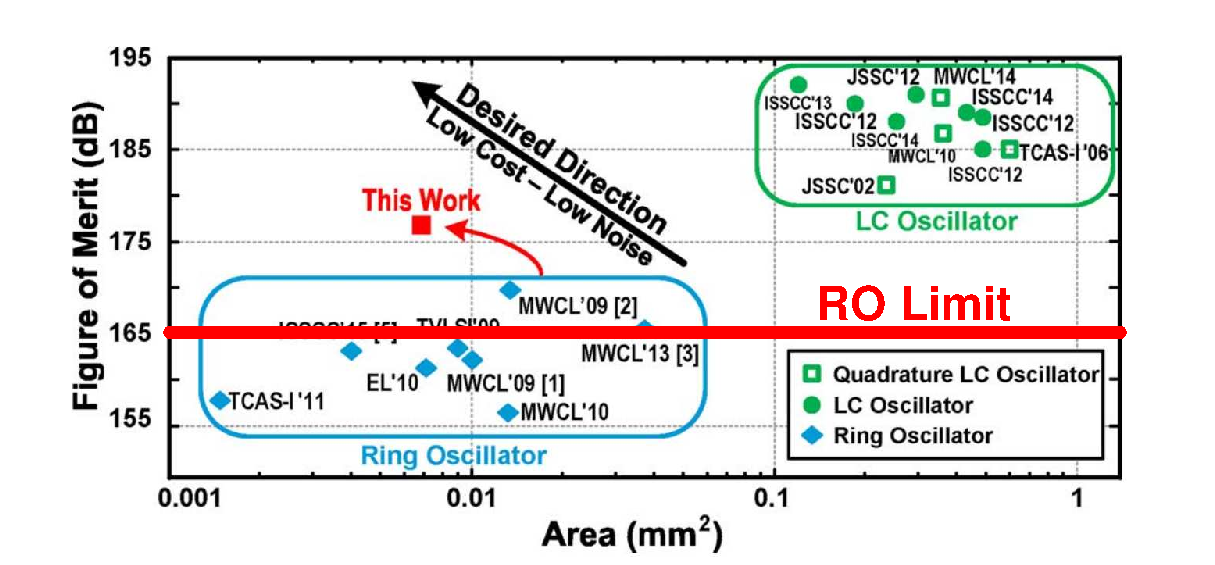
\includegraphics[width=0.75\textwidth, angle=0]{figs/ro_perf.pdf}



	\section{pres2}
		\flushleft
		\subsection{Initial simulation/modeling approach}
		\vspace{-.2em}
		\begin{itemize}
			\footnotesize
			\item Started writing Python code to simulate digital PLL.
			\begin{itemize}
				\footnotesize
				\item Most familiar for me (I have modelled CDRs in Python before).
				\item Simple to implement digital filters with Python Control Systems Library.
				\begin{itemize}
					\scriptsize
					\item Also - Convenient stability analysis.
				\end{itemize}
			\end{itemize}
			\footnotesize
			\item Decided starting point:
			\begin{itemize}
				\footnotesize
				\item Model DCO based on physical phase-noise limit of ring-oscillators. 
				\item Model loop filter as digital IIR second-order LPF (approximate second-order type-II analog PLL).
				\item Ideal divider and TDC.
			\end{itemize} 
			\item Investigate (to determine component requirements):
			\begin{itemize}
				\footnotesize
				\item Loop-BW to achieve PN requirements. Closed-loop sensitivity analysis:
				\begin{itemize}
					\scriptsize
					\item TDC phase noise significant at f<BW, determine limits for this. 
				\end{itemize}
			\end{itemize}
		\end{itemize}    
		\begin{itemize}
			\footnotesize
			\item Investigate (continued):
			\begin{itemize}
				\footnotesize
				\item Quantization, linearity impact of TDC \& DCO on phase noise.
				\begin{itemize}
					\scriptsize
					\item Determine number of bits required for each, and non-linearity limits.  
				\end{itemize}
				\item Loop filter implementations (IIR vs FIR), order \& type.
				\begin{itemize}
					\scriptsize
					\item Evaluate stability, lock time, operating region to meet requirements. 
				\end{itemize}
				\item Digital data path requirements to implement filter.
				\item Algorithm/state machine for handling continuity of fine/coarse DCO ranging. 
				\begin{itemize}
					\scriptsize
					\item Previous two lead to Verilog description.  
				\end{itemize}
			\end{itemize}
			\item \textbf{Final Outcomes:}
			\begin{itemize}
				\footnotesize
				\item Full design constraints for PLL components, sufficient to allow schematic-level implementation.
			\end{itemize}
		\end{itemize}    

		\subsection{Implementation in Cadence}
		\vspace{-.2em}
		\begin{itemize}
			\footnotesize
			\item When initial modeling/simulation satisfactory, translate design into a setup within Cadence.
			\begin{itemize}
				\footnotesize
				\item Implement using Verilog-A, ahdlLib components?
			\end{itemize}
			\footnotesize
			\item Will act as known-good test bench for testing transistor-level implementations of components in future design stages.
			\begin{itemize}
				\footnotesize
				\item Replace element by element until fully functioning at transistor level.
			\end{itemize}
		\end{itemize}    


	\section{pres4}
		\flushleft
		\subsection{Simulation approach}
		\vspace{-.2em}
		\begin{itemize}
			\footnotesize
			\item My current full-PLL simulations are not generally stable.
			\begin{itemize}
				\scriptsize
				\item Due to arbitrary choices for loop filter parameters not yielding a stable loop.				
				\item Next week plan is simulation / analysis / requirements definition of loop filter.
				\item Will have to address issue of phase wrapping, fixed point resolution.
			\end{itemize}
		\end{itemize} 	
		\vspace{-1.5em}
		\center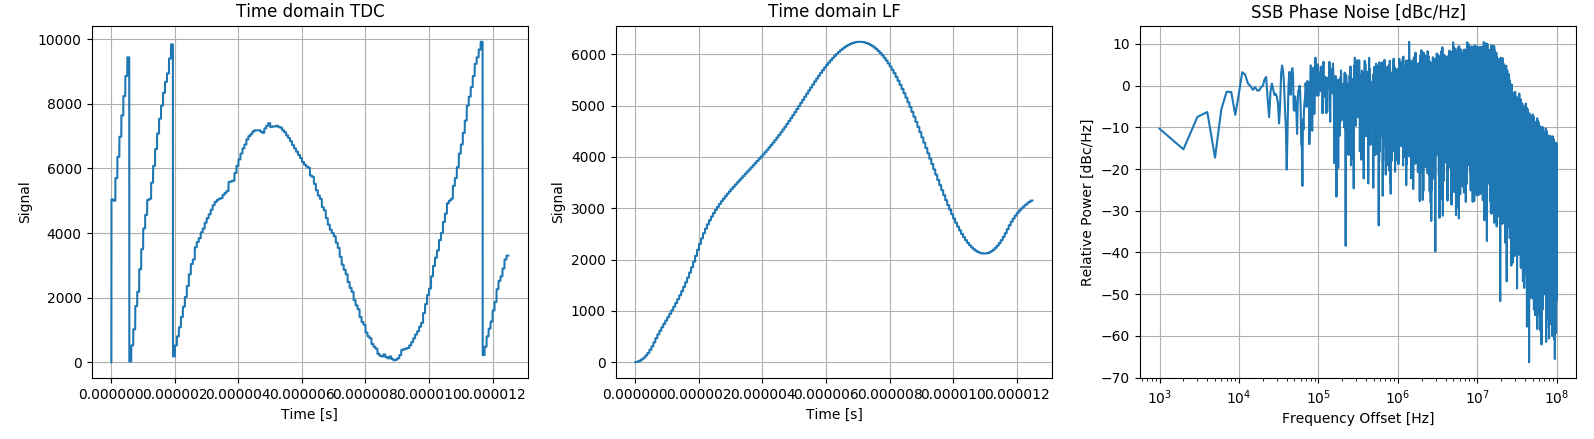
\includegraphics[width=0.75\textwidth, angle=0]{figs/unstable2.png}
		\vspace{-0.5em}
		\begin{itemize}
			\footnotesize
			\item Opted for mathematical-modelling of TDC, separate simulation of DCO.
			\begin{itemize}
				\scriptsize
				\item Found straightforward model for TDC phase noise from Michael Perrott of MIT.
				\item DCO simulation estimates quantization noise.
				\item Will resume with full PLL simulation for loop filter and remainder of modeling.
			\end{itemize} 

		\end{itemize}  

		\flushleft  
		\subsection{DCO performance criteria}
		\vspace{-.2em}
		\begin{itemize}
			\scriptsize
			\item Resolution set by frequency accuracy requirements, quantization noise.
			\item Quantization noise is manifested here as:
			\begin{itemize}
				\scriptsize			
				\item Reference spurs resulting from deterministic components of signal.
				\item A quasi-random noise signal when lock is achieved.
				\begin{itemize}
					\scriptsize			
					\item Results from stochastic toggling of $\sim$ 1 LSB of DCO tuning word to track low frequency variations.
					\item Rolloff of -20 dB/decade at low frequency (same as ring oscillator), -40 dB/decade at high frequencies.
				\end{itemize} 				
			\end{itemize} 
		\vspace{-1em}
		\center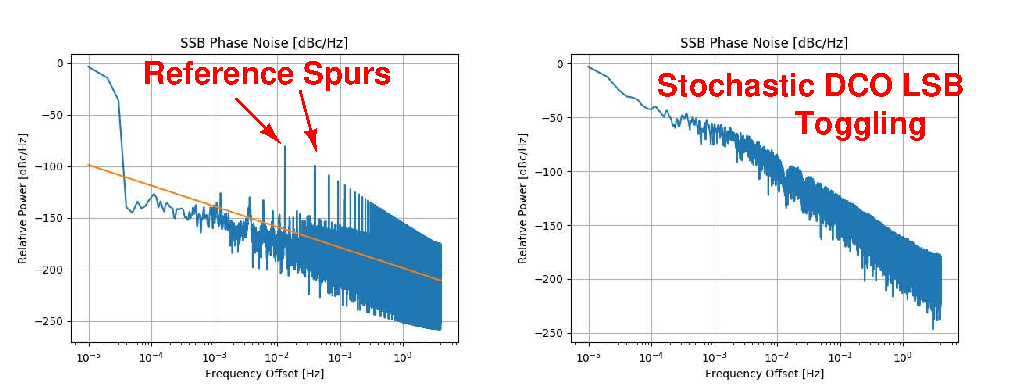
\includegraphics[width=0.7\textwidth, angle=0]{figs/quant_noise.pdf}
		\vspace{-0.5em}  
		\end{itemize}   

		\flushleft
		\subsection{DCO - reference spur requirements}
		\vspace{-.2em}
		\begin{itemize}
			\footnotesize
			\item Worst case reference spur level.
				\begin{itemize}
					\scriptsize			
					\item DCO tuning word toggling up/down 1 LSB every reference cycle.
				\end{itemize} 	
			\item With $f_0$ = 2.4 GHz, $f_{clk}$ = 16 MHz:
			\begin{itemize}
				\scriptsize			
				\item 52 kHz per LSB (i.e. $K_{DCO}$) is needed for a maximum -60 dBc reference spur level. 
			\end{itemize} 
		\end{itemize}  
		\vspace{-1em}
		\center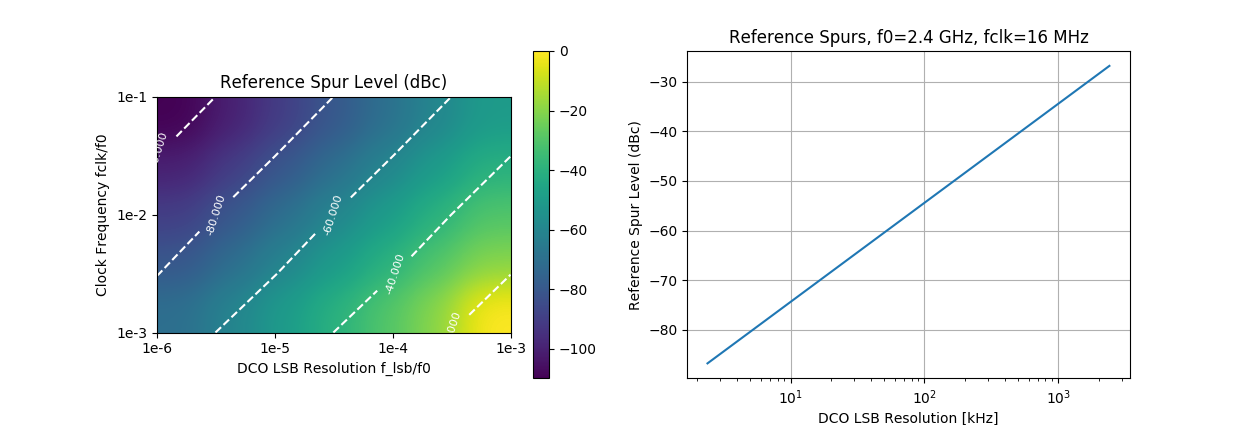
\includegraphics[width=1.0\textwidth, angle=0]{figs/refspur_level.png}
		\vspace{-0.5em}  

		\flushleft
		\subsection{DCO - steady state cap noise}
		% \vspace{-.2em}
		\begin{minipage}{7cm}
			\vspace{1em}
			\begin{itemize}
				\scriptsize
				\item In steady state, DCO tuning word will vary occassionaly by $\sim$ 1 LSB to track stochastic frequency changes.
				\begin{itemize}
					\tiny
					\item This generates noise and should be less than the thermal phase noise of DCO.		
					\item Very pessimistic estimate here (assumes abrupt frequency change). Abrupt frequency steps contribute 1/$\Delta f$ dependent component to phase noise.
				\end{itemize} 
				\item Theoretical ring oscillator phase noise limit from [2]:
				\tiny
				\begin{equation}
					PN_{min}(\Delta f)= 10\log 10\left(\frac{7.33k_BT}{P}\left(\frac{f_0}{\Delta f}\right)^2\right)
				\end{equation}
				\scriptsize
				\item If $f_0$ = 2.4 GHz, P = 50 $\mu$W, $\Delta f$= 1 MHz, T = 293K, $\rightarrow$ \textbf{PN < -84.7 dBc/Hz} from this noise process.
				\begin{itemize}
					\scriptsize			
					\item LSB resolution of \textbf{50 kHz} seems feasible. Will have to verify with full PLL sim to account for loop dynamics.
				\end{itemize} 
			\end{itemize}  
		\end{minipage}%
		% \hspace{-0.5cm}
		\begin{minipage}{5cm}
			% \vspace{-1.5em}
			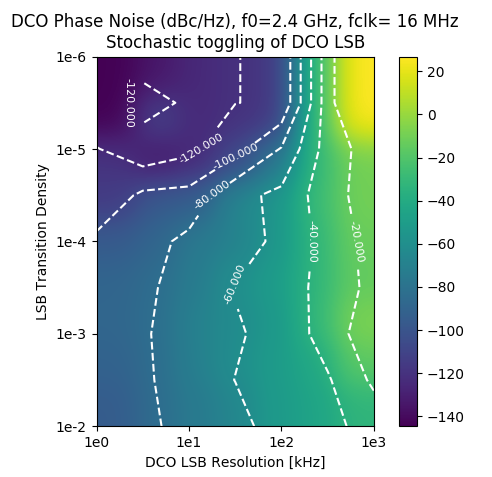
\includegraphics[width=1\textwidth, angle=0]{figs/lsb_stochastic_pn.png}
			% \vspace{-0.5em}  
		\end{minipage}%

		\flushleft
		\subsection{DCO - linearity and accuracy}
		\vspace{-.2em}
		\begin{itemize}
			\footnotesize
			\item Frequency accuracy.
				\begin{itemize}
					\scriptsize			
					\item Indeterminate IF assumed for wake up receivers, so accuracy not so critical.
					\item If RF bandwidth of receiver > PLL bandwidth, reasonable assumption is maximum frequency offset (accuracy) should be < PLL bandwidth.
					\item Current PLL bandwidth spec is 100 kHz, suggested 50 kHz LSB step from quantization noise analysis is sufficient?
					\begin{itemize}
						\scriptsize			
						\item This is assuming accuracy is tied to DCO resolution.
					\end{itemize} 
				\end{itemize} 	
			\item Linearity:
			\begin{itemize}
				\scriptsize			
				\item Integral non-linearity over the tuning DCO range is not important, so no spec for INL is suggested. Should be locally linear (constrains DNL).
				\item Monotonicity is essential, so must strictly have DNL < 1 LSB.
			\end{itemize} 
		\end{itemize} 

		\flushleft
		\subsection{TDC - phase noise model}
 		\begin{itemize}
			\scriptsize
			\item Based on a phase-domain model for PLL phase noise from Michael Perrot [1].

		\end{itemize}  

		\begin{minipage}{5cm}
			\tiny
			\begin{equation}
				S_{\phi,out}(f)= f_{clk}\cdot\left| 2\pi NG(f) \right|^2\cdot\frac{\Delta t_{del}^2}{12}
			\end{equation}
			\begin{equation}
				G(f)= \frac{A(f)}{1 + A(f)}
			\end{equation}
		\end{minipage}
		\begin{minipage}{6cm}
			% \vspace{-1em}
			\center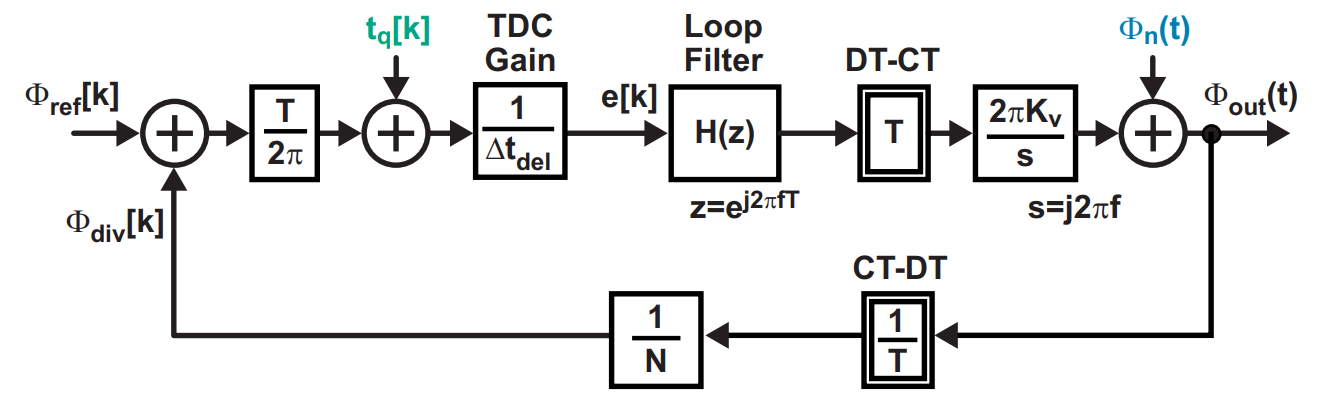
\includegraphics[width=1\textwidth, angle=0]{figs/pll_loop.png}
			% \vspace{-0.5em}
		\end{minipage}
 		\begin{itemize}
			\scriptsize
			\item $S_{\phi,out}(f)$ is the TDC phase noise component, N is the divider modulus, G(f) is the closed loop PLL transfer function, A(f) is the open loop transfer function, $\Delta t_{del}$ is the TDC time resolution.
			\item G(0) = 1, and G(f) $\approx$ 1 for f $\in$ [0, $f_{CBW}$], where $f_{CBW}$ is the closed loop bandwidth.

		\end{itemize}  

		\begin{itemize}
			\footnotesize
			\item Naive estimate for TDC time resolution:
			\begin{itemize}
				\scriptsize
				\item Phase noise flat within closed-loop bandwidth. This component dominates power of the integrated phase noise a PLL with low TDC-resolution.
				\item Use Residual frequency modulation equation and equation 2 (TDC phase noise) to estimate $\Delta t_{del}$. Integrate in f $\in$ [0, $f_{CBW}$]
			\end{itemize} 
			\begin{equation}
				\Delta f_{RFM} = 2\int_{f_a}^{f_b}f^2*PN(f)df
			\end{equation}
			\item With $f_{clk}$ = 16 MHz, N = 150 (for 2.4 GHz synthesis), $\Delta f_{RFM}$ < 107 kHz to meet BER requirement, and $f_{CBW}$ = 100 kHz. (PLL presumed to have very low TDC resolution)
 			\begin{itemize}
				\scriptsize			
				\item $\Delta t_{del}$ < 3.8 ns
				\item Phase noise of TDC below $f_{CBW}$ is -47.7 dBc/Hz
				\item Equates to minimum of 16.4 quantization steps for TDC (4.03 bits).
				\item Assumptions of high phase noise and low resolution appear valid.

			\end{itemize} 
		\end{itemize}  

	\section{pres5}
		\flushleft
		\subsection{This week}
		\begin{itemize}
			\footnotesize
			\item \textbf{Primary:} Loop analysis, requirements definition.
			\begin{itemize}
				\footnotesize
				\item Design open loop filter design to meet closed loop requirements.
				\begin{itemize}
					\item Dependent on DCO properties ($k_{DCO}$, $f_0$, tuning range).
					\item Difference equation implementing discrete time 2nd order IIR filter.
				\end{itemize} 
				\item Datapath requirements (fixed-point resolution)
			\end{itemize} 
		\end{itemize}  
		\flushleft
		\subsection{Next week} 
		\begin{itemize}
			\footnotesize
			\item \textbf{Primary:} Ideal component PLL implementation in Cadence, \color{red} continue loop filter work.
			\begin{itemize}
				\footnotesize
				\item Ideal component PLL implementation is not a lot of work.
				\item Loop filter very critical, spend more time on this.
				\begin{itemize}
					\footnotesize
					\item Need to make Verilog description of loop filter for simulation in Cadence.
				\end{itemize}
			\end{itemize} 
		\end{itemize}   
		\flushleft
		\subsection{Loop filter original attempt}
		\vspace{-.2em}
		\vspace{-0.5em}
		\center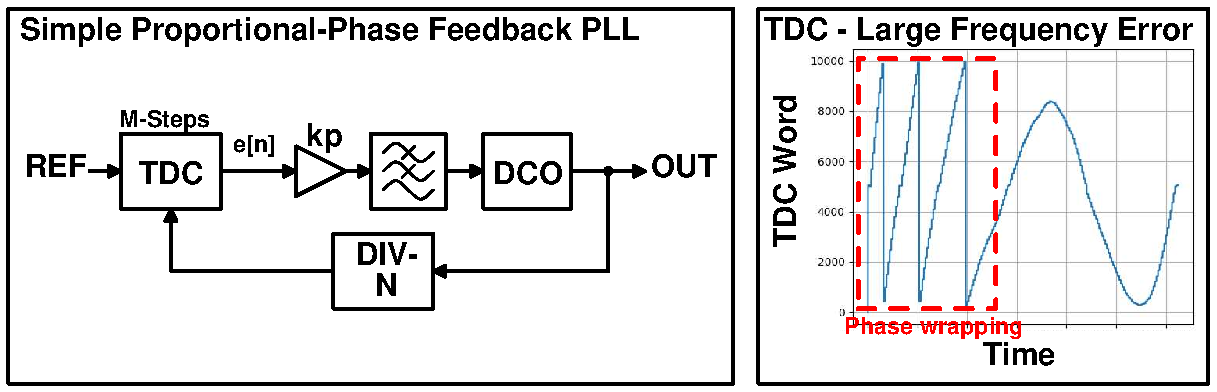
\includegraphics[width=0.75\textwidth, angle=0]{figs/phase_wrap.pdf}
		\vspace{-0.5em}
		\begin{itemize}
			\footnotesize
			\item Started with simple PLL loop with proportional-phase fed into loop filter (LF).
			\begin{itemize}
				\scriptsize
				\item Not stable at large frequency offset, due to frequency wrapping. At the TDC:
				\tiny
				\begin{equation}
					\Delta \phi = \frac{2\pi \Delta f T}{N} \rightarrow T_{wrap} = \frac{N}{\Delta f}
				\end{equation}
				\scriptsize
				\item Upon cold start, $\Delta f$ is expected to be up to 100 MHz, N=150 $\rightarrow T_{wrap} = $ 1.5 $\mu$s
				\begin{itemize} 
					\scriptsize
					\item $f_{wrap} \sim$  600 kHz, this is unstable with a loop bandwidth of 100 kHz.
				\end{itemize}
				\item Must opt for alternate loop structure.
			\end{itemize}
		\end{itemize} 	
		\flushleft
		\subsection{Loop filter new approach}
		\vspace{-0.5em}
		\center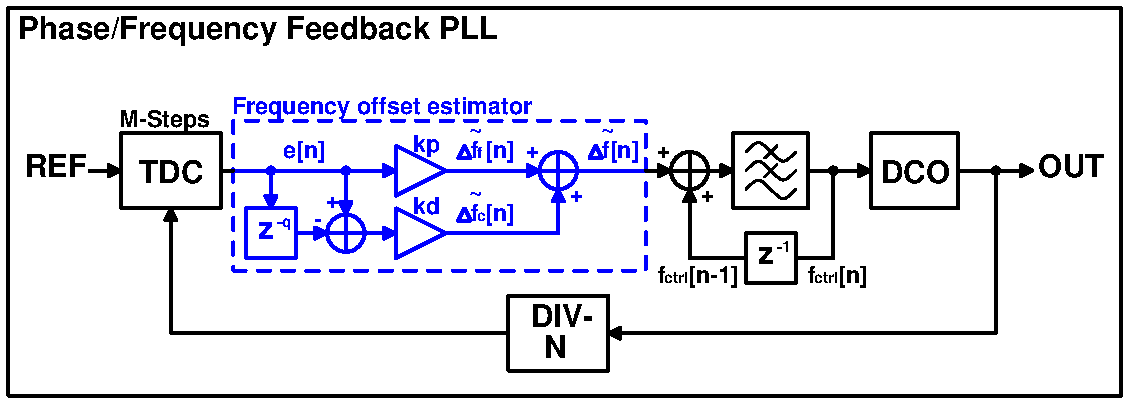
\includegraphics[width=0.75\textwidth, angle=0]{figs/more_advanced.pdf}
		\vspace{-0.5em}
		\begin{itemize}
			\footnotesize
			\item Two-fold approach: utilize propotional-phase and coarse frequency offset estimation in feedback.
			\begin{itemize}
				\scriptsize
				\item Coarse frequency estimator to handle high frequency offset (e.g. cold start-up).	
				\item Proportional-phase for near steady state. Acts like fine frequency estimator.
			\end{itemize}
			\item Offset estimates are summed with previous oscillator tuning word (OTW, also $f_{ctrl}$ here), then low passed filtered to yield new OTW. 
			\begin{itemize}
				\scriptsize
				\item Low pass filter loop keeps steady state.	
				\item Frequency estimator updates if any changes detected.
			\end{itemize}			
		\end{itemize} 	
		\flushleft
		\subsection{Coarse frequency estimation}
		\vspace{-0.5em}
		\center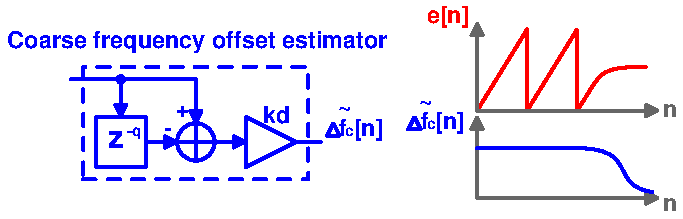
\includegraphics[width=0.5\linewidth, angle=0]{figs/coarse_est.pdf}
		\begin{itemize}
			\footnotesize
			\item \textbf{Coarse frequency estimation:} Given M-step TDC, outputting phase error signal e$_\phi$[n], and a divider modulus N
			\tiny
			\vspace{-1em}
			\begin{equation}
				\Delta \phi_{DCO}[n; q] = N\cdot\Delta \phi_{REF}[n] = 2\pi \frac{N}{M}\left( e_\phi[n]-e_\phi[n-q]\right ),\hspace{2em} \Delta \phi_{DCO}[n; q] = \Delta \omega_{DCO}[n]qT_{ref} = 2\pi q \frac{\Delta \tilde f_{DCO}}{f_{ref}}
			\end{equation}
			\vspace{-1em}
			\begin{equation}
				\Delta \tilde f_{c} =\Delta \tilde f_{DCO} = \frac{f_{ref}}{q}\frac{N}{M}\left( e_\phi[n]-e_\phi[n-q]\right )
			\end{equation}				
			\footnotesize	
			\item Is a discrete differentiator, with gain coeficient to convert $d\phi/dt$ to frequency. 
			\begin{itemize}
				\scriptsize
				\item Design logic to handle phase wrapping.	
				\item Useful in coarse frequency range calibration. Can detect fast if frequency offset too large.
				\item Delay q is used to increase frequency resolution. 
			\end{itemize}			
		\end{itemize} 
		\begin{itemize}
			\footnotesize
			\item Given DCO gain $K_{DCO}$, the required gain $K_d$ of the filter is:
			\tiny
			\vspace{-0.5em}
			\begin{equation}
				K_{d} = \frac{f_{ref}}{qK_{DCO}}\frac{N}{M}\left( e_\phi[n]-e_\phi[n-q]\right )
			\end{equation}				
			\footnotesize	
			\item Disable the coarse estimator if $e_\phi[n]-e_\phi[n-q]$ < some threshold:
			\begin{itemize}
				\scriptsize
				\item Offset small enough, allow to run as classical phase-detector mode.
			\end{itemize}	
		\end{itemize} 

		\flushleft
		\subsection{Loop filter Gain Coefficients}
		\vspace{-0.5em}
		\center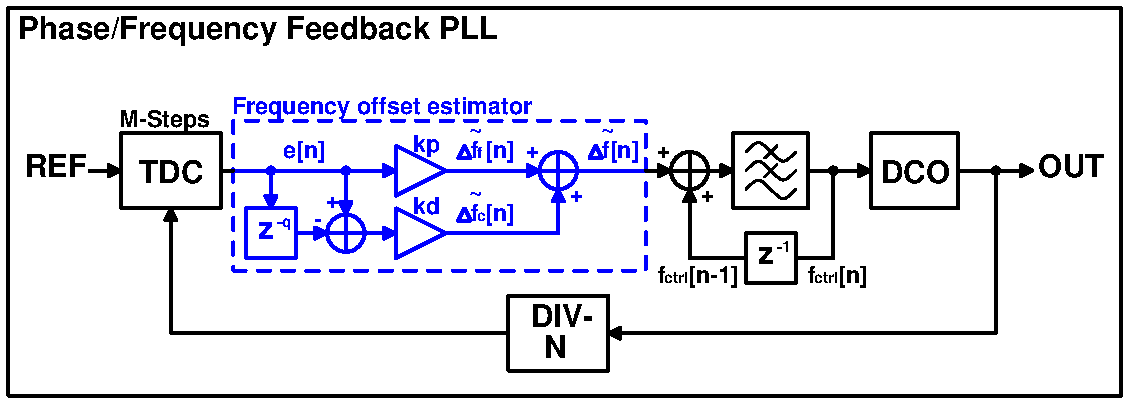
\includegraphics[width=0.75\textwidth, angle=0]{figs/more_advanced.pdf}
		% \vspace{-0.5em}
		\begin{itemize}
			\footnotesize
			\item When running in proportional-only feedback mode, the open loop gain $A(f)$ is:
			\tiny
			\begin{equation}
				A(f) = K_p \frac{M}{N}\frac{K_{LPF}}{s + \omega_{LPF} - K_{LPF}}\frac{2\pi K_{DCO}}{s}
			\end{equation}
			\footnotesize
			\item The closed loop gain is therefore (continuous):
			\tiny
			\begin{equation}
				G(f) =  \frac{A(f)}{1+A(f)}= \frac{2\pi M K_pK_{LPF}K_{DCO}/N}{s^2+s(\omega_{LPF - K_{LPF}})/N + 2\pi M K_pK_{LPF}K_{DCO}/N}
			\end{equation}	
		\end{itemize} 
		\begin{itemize}
			\scriptsize
			\item The form of a second order low pass filter is, with natural frequency $\omega_n$ and damping coefficient $\zeta$:
			\tiny
			\begin{equation}
				H_{LPF}(f) = \frac{\omega_n^2}{s^2 + 2\zeta\omega_ns + \omega_n^2}
			\end{equation}
			\scriptsize
			\item Setting $H_{LPF}(f) = G(f)$, equivalencies for $\omega_n$ and $\zeta$ are found:
			\tiny
			\begin{equation}
				\omega_n = \sqrt{2\pi M K_pK_{LPF}K_{DCO}/N}
			\end{equation}			
			\begin{equation}
				\zeta = \frac{\omega_{LPF - K_{LPF}}}{2\sqrt{2\pi MN K_pK_{LPF}K_{DCO}}}
			\end{equation}	
			\scriptsize
			\item The Butterworth closed loop response with 100 kHz bandwidth, $\omega_n \sim 2\pi\cdot 100 Khz$, $\zeta=0.707$.
			\item Coefficients $K_{LPF}$, $K_p$, $\omega_n$ can be solved computationally.
			\item Need to reformulate in Z-domain.
		\end{itemize} 	

		\flushleft
		\subsection{Coarse frequency calibration}
		\begin{itemize}
			\vspace{-0.25em}
			\scriptsize
			\item Ring oscillator DCOs will have large variation in frequency due to PVT variation.
			\item Use bank of coarse capacitance values to correct range of oscillator.
			\item Coarse frequency estimator used in this calibration.  DCO is has a fine range of $\Delta f_{fine}$.
		\end{itemize} 	
		\vspace{-0.25em}
		\scriptsize
		\textbf{Coarse frequency tuning state machine} (as pseudo-code)
			\begin{enumerate}
				\scriptsize
				\item $C_{tune}$ = $C_{opt}$ = 0;\hspace{1em} LE = $\Delta f_{fine}$		
				\item Reset PLL
				\item Estimate Frequency offset $\rightarrow \tilde f_{offset}$
				\vspace{-0.2em}
				\item \textbf{If} abs($\tilde f_{offset}$ - $\Delta f_{fine}/2$)  \textbf{<} LE: \hspace{1em}\color{teal} // Centers fine tuning range around target frequency
				\color{black}
				\begin{itemize}
					\scriptsize
					\item LE = abs($\tilde f_{offset}$ - $\Delta f_{fine}/2$)
					\item $C_{opt}$ = $C_{tune}$
				\end{itemize}	
				\item \textbf{If} $C_{tune}$ \textbf{==} $C_{max}$: \textbf{Goto} 8		
				\item $C_{tune}$ += 1
				\item \textbf{Goto} 2
				\item $C_{tune}$ = $C_{opt}$; \textbf{End}
			\end{enumerate}
 

	% % % % % % % % % % % % % % % % % % % % % % % % % % % % % % % % % % % % 
	% References
    \pagebreak

	\bibliographystyle{plain}
	\bibliography{mybib}{}


	% % % % % % % % % % % % % % % % % % % % % % % % % % % % % % % % % % % % 
	% Appendix
	\pagebreak
	\appendix

	\section{Appendix - Schedule}
	\begin{table}
		\footnotesize
		\def\arraystretch{1.5}		
		\setlength\arrayrulewidth{0.75pt}
		\setlength{\tabcolsep}{1em} % for the horizontal padding
		\begin{tabular}{|l|l|l|l|}
			\hline 
			\rule[-1ex]{0pt}{2.5ex} \cellcolor{gray!40}\textbf{Week Number} & \cellcolor{gray!40}\textbf{Dates} &\cellcolor{gray!40}\textbf{Tasks} & \cellcolor{gray!40}\textbf{Outcomes}\\ 
			\hline 
			\rule[-1ex]{0pt}{2.5ex} \cellcolor{red!20}\textbf{36}& \cellcolor{red!20}2.9 - 8.9 & \cellcolor{red!20}Review PLL Design & \cellcolor{red!20}Refreshed Knowledge\\ 
			\hline 
			\rule[-1ex]{0pt}{2.5ex} \cellcolor{red!20}\textbf{37}& \cellcolor{red!20}9.9 - 15.9 & \cellcolor{red!20}Modeling/simulation (set up) & \cellcolor{red!20}--\\ 
			\hline 
			\rule[-1ex]{0pt}{2.5ex} \cellcolor{red!20}\textbf{38}& \cellcolor{red!20}16.9 - 22.9 & \cellcolor{red!20}Modeling/simulation &\cellcolor{red!20} TDC/DCO Requirements\\ 
			\hline 
			\rule[-1ex]{0pt}{2.5ex} \cellcolor{green!20}\textbf{39}& \cellcolor{green!20}23.9 - 29.9& \cellcolor{green!20}Modeling/simulation& \cellcolor{green!20}Loop Filter/Digital Algorithms\\ 
			\hline 
			\rule[-1ex]{0pt}{2.5ex} \cellcolor{blue!20}\textbf{40}& \cellcolor{blue!20}30.9 - 6.10& \cellcolor{blue!20}Modeling/simulation& \cellcolor{blue!20}\color{red}{\textbf{Loop filter,}} \color{black}{Ideal implementation in Cadence}\\ 
			\hline 
			\rule[-1ex]{0pt}{2.5ex} \textbf{41}& 7.10 - 13.10& Circuit Research & DCO/Divider topologies\\ 
			\hline 
			\rule[-1ex]{0pt}{2.5ex} \textbf{42}& 14.10 - 20.10& Circuit Research & TDC/other topologies\\ 
			\hline 
			\rule[-1ex]{0pt}{2.5ex} \textbf{43}& 21.10 - 27.10& Circuit Implementation& Digital logic (schematic)\\ 
			\hline 
			\rule[-1ex]{0pt}{2.5ex} \textbf{44}& 28.10 - 3.11& Circuit Implementation& DCO (schematic)\\ 
			\hline 
			\rule[-1ex]{0pt}{2.5ex} \textbf{45}& 4.11 - 10.11& Circuit Implementation& Divider/other (schematic)\\ 
			\hline 
			\rule[-1ex]{0pt}{2.5ex} \textbf{46}& 11.11 - 17.11& Circuit Implementation (TDC)& \\ 
			\hline 
			\rule[-1ex]{0pt}{2.5ex} \textbf{47}& 18.11 - 24.11& Circuit Implementation (TDC)& TDC (schematic)\\ 
			\hline 
			\rule[-1ex]{0pt}{2.5ex} \textbf{48}& 25.11 - 1.12& Full Circuit testing & Testbenches, find bugs, design fixes\\ 
			\hline 
			\rule[-1ex]{0pt}{2.5ex} \textbf{49}& 2.12 - 8.12& Full Circuit testing& Design Fixes/iteration\\ 
			\hline 
			\rule[-1ex]{0pt}{2.5ex} \textbf{50}& 9.12 - 15.12& --& --\\ 
			\hline 
		\end{tabular}
		\begin{flushleft}\textbf{Legend:} \colorbox{red!20}{\textbf{Done}} \colorbox{green!20}{\textbf{Current}}  \colorbox{blue!20}{\textbf{Revised}}
		% *I will write the report simultaneously with the work.
		\end{flushleft}
		% \caption{Assigned specifications for branch line hybrid design.}
		% \label{asgn_specs}
	\end{table}  

	\section{Appendix - Code}


    \begin{lstlisting}[language={Python}, caption={excode}, label={Blabla}]
#################################################################
# Simulation loop
#################################################################

t0 = time.clock()
for n in range(SAMPLES)[1:]:
    clk_out[n] = clk.update()
    tdc_out[n] = TDC_SCALE*((TDC_OFFSET+tdc.update(clk=clk_out[n-1], xin=div_out[n-1]))%TDC_STEPS)
    lf_out[n]  = lf.update(xin=tdc_out[n-1], clk=clk_out[n-1])
    osc_out[n] = dco.update(lf_out[n-1])
    div_out[n] = div.update(osc_out[n-1], DIV_N)
tdelta = time.clock() - t0
print("\nSimulation completed in%f s"%tdelta)
    \end{lstlisting}


\end{document}